\documentclass{Beautybook}
\usepackage{stys/BBCmds}


% 自定义head的颜色
\definecolor{bg}{HTML}{e0e0e0}
\definecolor{fg}{HTML}{455a64}
\colorlet{outermarginbgcolor}{bg}
\colorlet{outermarginfgcolor}{fg}
\colorlet{framegolden}{fg}
\colorlet{framegray}{黛绿!5}


\begin{document}

    %%%%%%%%%%%%    一些基本参数配置      %%%%%%%%%%%%
    % \thispagestyle{empty}               %% 这个不能去,不然后面的左右书签会乱码
    \title{BeautyBook 模板使用说明}
    \subtitle{原作者:陆世龙}
    \edition{First Edition}
    \bookseries{Illustrations On a \LaTeX{} Template---Beautybook}
    \author{Eureka}
    \pressname{Springer}
    \presslogo{Inner_Pics/Springer_Logo.png}
    \coverimage{Inner_Pics/TitleCover.png}
    \makecover
    \begin{Introduction}
        书籍内容说明填写处,可以用于说明书籍的基本内容,作者的基本情况等...
    \end{Introduction}
    
    \frontmatter
    \pagenumbering{Roman}
    \thispagestyle{empty}
\addcontentsline{toc}{chapter}{前言}
\chapter*{前言}
这个是前言,这里是前言测试内容

\vspace*{3em}
\phantom{\rule{.8\linewidth+.1em}{0pt}} ---- Eureka\\ 
\phantom{\rule{.8\linewidth+.1em}{0pt}}  \today

% 后面这部分用于放置生成多余的空白页面
\begin{center}
    \vfill
    \thepage
\end{center}
\let\cleardoublepage\clearpage




    \thispagestyle{empty}
    \definecolor{maincolor}{HTML}{8B8989}
    \tableofcontents
    \mainmatter

    \pagenumbering{arabic}
    % \setcounter{page}{1}
    \partimage{Inner_Pics/Part_Back_Image.png}
    %%%%%%%% 下面自由发挥 %%%%%%%%%%




%%%%%%%%    开始真正的写作   %%%%%%%%
\partabstract{%
    \hspace{2em}这里是每一个part的开篇说明内容,你可以使用命令\textbackslash 来
    设置每个part开篇你内容的背景图片。注意:你的partabstract必须在声明part
    前就声明,不然你的abstract并不会被读取。
}
\part{新手模板入门}


\chapter{常见内容}\index{索引变量}
\section{模板的基本结构}
\subsection{基本的文档结构}

本模板在BeautyBook的基础上进行了重新设计,模板源码结构如下:
\begin{figure}[!htb]
    \centering
    \rotatebox{-90}{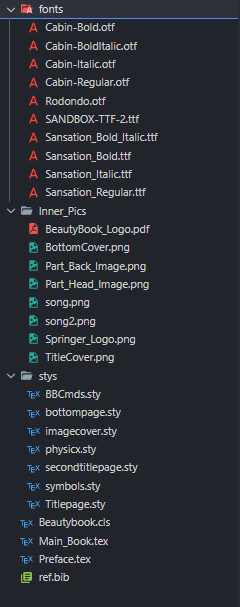
\includegraphics[scale=.8]{./Pics/Struct.png}}
    \caption{模板源码结构}
    \label{模板源码结构}
\end{figure}

\begin{enumerate}
    \item part
    \item chapter
    \item section
    \item subsection
\end{enumerate}

所以本模板的基本调用格式为如下:

\clearpage
\noindent\rule{.9\linewidth}{2pt}

\begin{verbatim}
\documentclass{Beautybook}
\usepackage{stys/BBCmds} 

\begin{document}
    %%%%%%%%%%%%    一些基本参数配置      %%%%%%%%%%%%
    % \thispagestyle{empty}    %% 这个不能去,不然后面的左右书签会乱码
    % 然后配置好如下的参数
    \title{}
    \subtitle{}
    \edition{First Edition}
    \bookseries{}
    \author{}
    \pressname{}
    \presslogo{}
    \coverimage{}
    \makecover
    \begin{Introduction}
        书籍内容说明填写处,可以用于说明书籍的基本内容,作者的基本情况等...
    \end{Introduction}
    
    \frontmatter
    \pagenumbering{Roman}
    \thispagestyle{empty}
\addcontentsline{toc}{chapter}{前言}
\chapter*{前言}
这个是前言,这里是前言测试内容

\vspace*{3em}
\phantom{\rule{.8\linewidth+.1em}{0pt}} ---- Eureka\\ 
\phantom{\rule{.8\linewidth+.1em}{0pt}}  \today

% 后面这部分用于放置生成多余的空白页面
\begin{center}
    \vfill
    \thepage
\end{center}
\let\cleardoublepage\clearpage




    \thispagestyle{empty}
    \definecolor{maincolor}{HTML}{8B8989}
    \tableofcontents
    \mainmatter

    \pagenumbering{arabic}
    % \setcounter{page}{1}
    \partimage{Inner_Pics/Part_Back_Image.png}
    %%%%%%%% 下面自由发挥 %%%%%%%%%%

    %% 你自己的内容

    \refandindex[可选说明]{BottomCover.png}
\end{document}
\end{verbatim}


\clearpage
\subsection{图片}
本模板的图片主要分为两类:
\begin{itemize}
    \item 模板必须的图片,位于Inner\_Pics内
    \item 作者自己组织文件夹进行图片管理,不要与模板内置模板内置图片文件夹
        Inner\_Pics冲突
\end{itemize}

\subsection{说明}
本模板的{\bf 说明}内容包含两部分:

\begin{itemize}
    \item Introduction环境
    \item \textbackslash refandindex命令
\end{itemize}

第一部分Introduction环境,放在前言之前。
这部分的内容主要放在Introduction环境内部,用于说明这个书籍的一些情况等
第二部分refandindex命令接受一个参数用于在封底输出一些本书的总结信息

\subsection{Preface}
其实就是一个单独的Preface.tex文件,你只需要根据自己的实际情况
在这个文件中增加你需要的内容即可。可以是一些你自己写的这本的的一些基本情况,
也可以是你对这本书读者的敬告 ...这个{\bf 前言}里面有一个默认参数:默认时间为当天。

{\bf 但是注意:}一点要在tableofcontents之前添加


\subsection{左右书签}
本部模板中的左右书签位置设定如下:在奇数页的{\bf 右侧},在偶数页的{\bf 左侧}。
而且默认在{\bf chapter}所在的页不显示。

\section{颜色配置}
本模板的颜色是可以自由配置的,可以配置的颜色参数如下:
\begin{verbatim}
\definecolor{bg}{HTML}{e0e0e0}
\definecolor{fg}{HTML}{455a64}
\colorlet{outermarginbgcolor}{bg}
\colorlet{outermarginfgcolor}{fg}
\colorlet{framegolden}{fg}
\colorlet{framegray}{黛绿!5}
\end{verbatim}

\section{数学环境}
下面是一些常用的定义好的数学环境
\begin{enumerate}
    \item definition
    \item theorem
    \item lemma
    \item proposition
    \item example
    \item corollary
\end{enumerate}

上述的命令还有自己的简写形式
\begin{enumerate}
    \item defi
    \item thm
    \item lem
    \item prop
    \item exam
    \item cor
\end{enumerate}

另外两个常用的环境
\begin{enumerate}
    \item fancybox--复古边框
    \item remark--备注
\end{enumerate}

\vspace*{2em}
\begin{warning}
    注意:如果你安装了mtpro2宏包,那么就取消BBCmds.sty中第39行左右的那个注释.
     同时还需要注释掉mtpro2.sty文件中的关于 Bbbk命令的定义。

    \begin{center}
        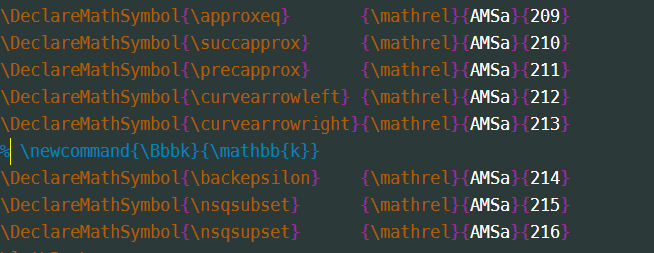
\includegraphics[scale=.6]{./Pics/Bbbk.png}
    \end{center}
\end{warning}

\clearpage
\subsection{完整数学环境}
\begin{definition}[][芽][def:芽]
    芽是定义在拓扑空间上函数集合的一种等价关系.
    定义在拓扑空间上的两个函数$f$和$g$,在点$x$处属于同一支芽,
    当且仅当存在一个开集$S$,使得$S$包含点$x$,且在$S$上$f$和$g$的函数值处处相等.

    一个复杂的公式

    \begin{align*}
        \lim _{\mathop{x \rightarrow 0^{+}}\limits_{y \rightarrow+\infty}}
        \frac{\displaystyle\sum_{n=1}^{\infty} \frac{(-1)^{n-1}}{n} \sum_{m=0}^{\infty} \frac{1}{n 2^{m}+1} \int_{0}^{x^{2}} \frac{\pi(\sqrt[4]{1+t}-1) \sin t^{4}}{\displaystyle\sum_{n=1}^{\infty} \frac{((n-1) !)^{2}(2 t)^{2 n}}{(2 n) !} \int_{0}^{1} \frac{(1-2 x) \ln (1-x)}{x^{2}-x+1} \mathrm{~d} x} \mathrm{~d} x}
        {x^{2}(x-\tan x) \ln \left(x^{2}+1\right)\left[\left(\frac{2 \arctan \frac{y}{x}}{\pi}\right)^{y}-1\right]}=\frac{27}{32}
    \end{align*}
\end{definition}

\begin{theorem}
    设$[f]\in\mathscr{F}_p$,对于包含$p$的容许坐标卡$(U,\varphi_U)$,令
    \begin{equation*}
    F(x^1,\cdots,x^n)=f\circ\varphi_U^{-1}(x^1,\cdots,x^n),
    \end{equation*}
    则$[f]\in\mathscr{H}_p$当且仅当
    \begin{equation*}
    \frac{\partial F}{\partial x^i}\Bigg|_{\varphi_U(p)}=0,\quad 1\leqslant t\leqslant n.
    \end{equation*}
\end{theorem}


\subsection{简写数学环境}
\begin{thm}
    \begin{enumerate}[label=(\arabic*),font=\upshape]
        \item 给定 $M,N$ 为两个 $n$维光滑流形且 $f$是从 $M$到 $N$的光滑映射.\cite{吴大任1979微分几何讲义}
        \item 在 $M$上一点 $p$处, $f$诱导的切映射 $f_*\colon T_p (M)\to T_{f(p)}(N)$是同构.
    \end{enumerate}
    则存在一点$p$在 $M$中的邻域 $U$, 使得 $V=f(U)$为 $f(p)$在 $N$中一邻域且 $f|_U\colon U\to V$是可微同胚.
\end{thm}

\begin{defi}
     这个是definition环境的简写形式
\end{defi}

\begin{cor}
    这是一个简略的 corollary环境
\end{cor}

\begin{lem}
    这是一个简略的 lemma 环境
\end{lem}

\begin{exam}
    这是一个简略的 example 环境
\end{exam}

\begin{prop} 
    这是一个简略的 proposition 环境
\end{prop}

\clearpage
\subsection{常用的两个盒子}
\begin{remark}
    这是一个注释
\end{remark}

\begin{fancybox}
    \textbf{\textcolor[rgb]{0.88,0.15,0.33}{看懂与撰写证明的方法技巧}}
    \begin{description}
        \item[\textbf{Step I.}] \textbf{理清证明的全局思维脉络 (化整为零)}~
        结合大纲、思维导图、逻辑组织架构图、树状图等等思维组织形式来把握整理整个证明
        流程的思路历程及关键环节、步骤,
        以及疏通条件与结论之间起桥梁作用的各个中间站点,明确它们的职能与权重。
        \item[\textbf{Step II.}] \textbf{斟酌微观的技术细节 (微观操作)}~
        透过回顾知识点、联想概念以及理论关联性来琢磨各个职能各异、
        权重参差的中间站点之间的联络方式,从而将其中的技术难点和微观层面的技术细节一一
        抠弄出来解决。
    \end{description}
\end{fancybox}



\section{参考文献和索引}

要使用参考文献,只需要把你的参考文献保存在{\bf 主文件同路径}下即可,
而且你的参考文献的名字只能为:{\bf ref.bib}.

至于怎么引用,引用的格式如下
\begin{verbatim}
    文本\cite{key}
\end{verbatim}

最后就是打印参考文献列表,使用如下的命令:
\begin{verbatim}
    \refandindex{文本}
\end{verbatim}

至于什么是索引,
其实就是把之前出现的名词等意义列举在最后,方便查找。这个sumary有一个可选参数,
具体语法:
\begin{verbatim}
        文本\index[说明文本]
\end{verbatim}

\section{编译方法}
文件的编译命令顺序如下:
\begin{enumerate}
    \item xelatex --shell-escape Main\_Book.tex
    \item biber Main\_Book (不用加拓展名)
    \item xelatex --shell-escape Main\_Book.tex
    \item xelatex --shell-escape Main\_Book.tex
\end{enumerate}


\partabstract{\hspace{2em}这一节的内容主要是关于模板的拓展到的,读者应该确保自己明白每个命令的含义}
\part{模板拓展}
\chapter{环境}

\section{环境添加}

下面是一个attention环境,使用tcolorbox宏包生成。

\vspace*{2em}
\begin{attention}[colbacktitle=green]{Attention}
    这是一个attention环境,用于高亮提醒标记
\end{attention}






\section{表格环境}
其实主要就是使用 $\textbackslash sptab\{Letters\}$ 来让字母填充在表格的背景中

\begin{center}
\begin{tabular}{|c|c|c|}\hline
    A & B & C\\\hline
    \sptab{A}{\lipsum[1]} & \sptab{B}{\lipsum[2]} & \sptab{C}{\lipsum[3]}\\\hline
\end{tabular}
\end{center}


\clearpage
\subsection{一个轮廓感很强的box}

这个colorbox的轮廓感很强,使用用于制作一个常用的提示环境

\begin{tcolorbox}[enhanced,size=small,sharp corners,
    colback=green!10,colframe=green!50!black,
    boxrule=1mm,titlerule=0mm,
    title=My title,center title,fonttitle=\bfseries,
    underlay={\tcbvignette{size=1mm,inside node=frame,
    raised color=green!50!black}}]
    This is a tcolorbox.
\end{tcolorbox}


\section{simbox环境}

一个有破缺边框的盒子, 演示效果如下:

\begin{simbox}[title=My unbroken box]
    \lipsum[1]
\end{simbox}


\section{一个表示警告的盒子}
这个盒子是很常见的,但是往往很难在其余的地方看到它的构造方法,下面给出它的一个构造
方法:

\begin{warning}
这个里面的内容表示警告

\lipsum[2]
\end{warning}



\refandindex[这个参数是可选的,这里可以添加一点的说明,类似于每本书的备注之类的]{BottomCover.png}



\end{document} 